%% go to the website http://en.wikibooks.org/wiki/LaTeX For Help 
\documentclass[11.5pt]{article}
%Math Related Packages
\usepackage{mathtools}
\usepackage{amsmath}
\usepackage{amsfonts}
\usepackage{amssymb}
\usepackage{relsize}
% Pseudocode Packages
\usepackage{algorithm}
\usepackage{algpseudocode}
\usepackage[colorinlistoftodos]{todonotes}
% Automata/Graph Packages
\usepackage{tikz}
\usepackage{pgf}
\usetikzlibrary{arrows,automata}
\usepackage[latin1]{inputenc}
\usetikzlibrary{automata,positioning}
%%%Formatting Options for Pages
%\usepackage[a4paper,left=2cm,right=2cm]{geometry} %Change Margins
\usepackage[colorlinks=true, allcolors=blue]{hyperref} % adds hyperlinks
\usepackage{listings}
\usepackage{multicol}
\usepackage{perpage}
\MakePerPage{footnote}
%%%Graphics Packages and Caption Tools
\usepackage{graphicx}
\usepackage{fullpage}
\newcounter{Figure} 
\setcounter{Figure}{1}
\usepackage{slashbox}
\usepackage{ulem}
\usepackage{csvsimple}
%%%Colors Package with Custom Defined Colors
\usepackage{color}
\usepackage{colortbl}
\definecolor{Gray}{gray}{0.9}
\definecolor{codegreen}{rgb}{0,0.6,.2}
\definecolor{codegray}{rgb}{0.5,0.5,0.5}
\definecolor{codepurple}{rgb}{0.58,0,0.82}
\definecolor{backcolor}{rgb}{0.94,0.94,1}
\definecolor{light-gray}{gray}{0.55}
%%Custom Functions and Commands
\newcommand\indentFour{\indent\indent\indent\indent}
\newcommand\indentThree{\indent\indent\indent}
\newcommand\indentTwo{\indent\indent}
\newcommand\tab{\ \ \ }
\newcommand\proof{\setcounter{equation}{0}\hfill\fbox{\rule{.02in}{0pt}\rule[0ex]{0pt}{.5ex}}}
%%Color Commands
\newcommand\BLK{\color{black}}
\newcommand\GRY{\color{Gray}}
\newcommand\BLU{\color{blue}}
\newcommand\blu{\color{CornflowerBlue}}
\newcommand\RED{\color{red}}
\newcommand\red{\color{RubineRed}}
\newcommand\ORG{\color{BurntOrange}}
\newcommand\org{\color{Peach}}
\newcommand\GRN{\color{ForestGreen}}
\newcommand\grn{\color{LimeGreen}}
\newcommand\PRP{\color{RoyalPurple}}
\newcommand\prp{\color{DarkOrchid}}
%%Math Commands
\newcommand{\Lbra}{\left\langle}
\newcommand{\Rbra}{\right|}
\newcommand{\Rket}{\right\rangle}
\newcommand{\Lket}{\left|}
\newcommand{\bra}[1]{\Lbra #1 \Rbra}
\newcommand{\ket}[1]{\Lket #1 \Rket}
\newcommand{\braket}[1]{\Lbra #1 \Rket}
\newcommand{\Exists}{\ \exists \ }
\newcommand{\Forall}{\ \forall \ }
\newcommand{\abs}[1]{\left| #1 \right|}
\newcommand{\Frac}[2]{\left(\frac{#1}{#2}\right)}
\newcommand{\Mat}[1]{\left[\begin{matrix} #1 \end{matrix}\right]}
\newcommand{\vhi}{\varphi}
\newcommand{\R}{\ \mathbb{R}}
\newcommand{\C}{\ \mathbb{C}}
\newcommand{\N}{\ \mathbb{N}}
\newcommand{\Z}{\ \mathbb{Z}}
\newcommand{\I}{\ \mathbb{R/Q}}
\newcommand{\x}{\mathrm{x}}
\newcommand{\mbf}[1]{\mathbf{#1}}
\newcommand{\Dpart}[2]{\frac{\partial #1}{\partial #2}}
\DeclarePairedDelimiter{\ceil}{\lceil}{\rceil}
\newcommand{\U}{\underline}
%Numbering
\newcounter{graphics}
\newcounter{tables}
%For coding
\lstdefinestyle{small}{
    backgroundcolor=\color{backcolor},   
    commentstyle=\color{codegreen},
    keywordstyle=\color{blue},
    numberstyle=\tiny\color{codegray},
    stringstyle=\color{codepurple},
    basicstyle=\footnotesize,
    breakatwhitespace=false,         
    breaklines=false,                 
    captionpos=b,                    
    keepspaces=false,                 
    numbers=left,                    
    numbersep=5pt,                  
    showspaces=false,                
    showstringspaces=false,
    showtabs=false,                  
    tabsize=4
}
%\lstinputlisting[language=Matlab]{cub_spline.m} %Use this to add code
\renewcommand{\abstractname}{Abstract}
\begin{document}
\title{MAT 128C - Program \# 2 Molecular Dynamics}
\author{Douglas Sherman, Aaron Millstein, Doug Kubota}
\date{June 2nd, 2017}
\maketitle
\rule{\textwidth}{1pt}
\lstset{style=small} %set code style, see preamble

\section{Introduction}
\paragraph{}
We propose a simulation of $N$ particles in a box with periodic boundary conditions (torus) by following Newton's Law of Motion based on the Leonard Jones potential energy function of
\begin{align} \label{eq:Potential}
E(r_{ij}) = 4\epsilon \left( \Frac{A}{r_{ij}}^12 - \Frac{B}{r_{ij}}^6\right) 
\end{align}
for some constants $\epsilon,A,$ and $B$ due to the particles in question. Newton's Law $\vec{F}=m\vec{a}$ with (\ref{eq:Potential}) gives us the differential equation as
\begin{align} \label{eg:FMA}
-\frac{dE}{dr}&=m\frac{d^2r}{dt^2}\notag \\ 
\iff 4\epsilon\left( 12\Frac{A}{r_{ij}}^{13} - 6\Frac{B}{r_{ij}}^7\right) &= m \frac{d^2r}{dt^2}
\end{align}
This study considers Argon atoms with a Van der Waals radius of $\sigma := 3.4 \dot{A}$ and simplify the problem as $A= B = \sigma$ and $\epsilon = \sigma = 1$. Thus we obtain $dE/dr$ as 
\begin{align*}
f_{ij}:= \frac{dE}{dr_{ij}} = 24\left(\frac{2}{r_{ij}^{13}} - \frac{1}{r_{ij}^7}\right)
\end{align*}

\section{Results}
\paragraph{2.1}\textbf{Simulate the Molecular Dynamics of $\mbf{N}$ particles in an $\mbf{L\times L}$ torus.}\\
\paragraph{}
We initialize the system with $N$ particles and assign initial velocities given by $v_0*\nu$ where $\nu$ is random Gaussian scale factor. Then using the potential function above we compute the acceleration at each $\Delta t$ interval as the sum of all the forces applied to each particle by the remaining $N-1$ particles. We compute the $x$ and $y$ components seperately using the geometry of the system as
\begin{align*}
f_{ij,x} &= f_{ij}\cos \theta = f_{ij} \frac{x_j - x_i}{r_{ij}}\\
f_{ij,y} &= f_{ij}\sin \theta = f_{ij} \frac{y_j - y_i}{r_{ij}}
\end{align*}
\pagebreak
\paragraph{}
The following illustrates the evolution of a system using $N=20, v_0 = 20, \Delta t = 0.01,$ and $L=5$. 
\begin{center}
\begin{tabular}{ccc}
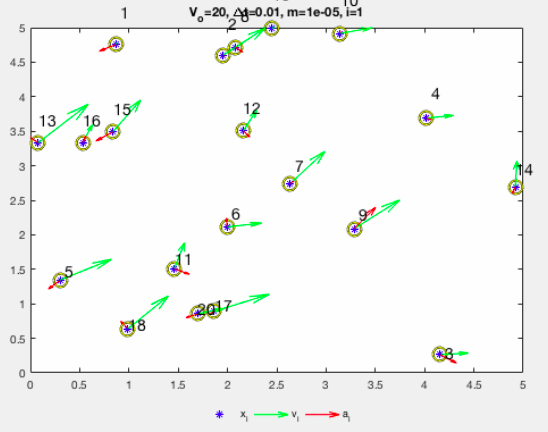
\includegraphics[width = 2in]{1.png}&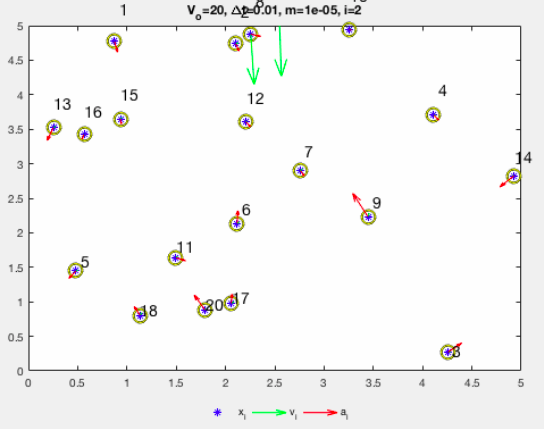
\includegraphics[width = 2in]{2.png}&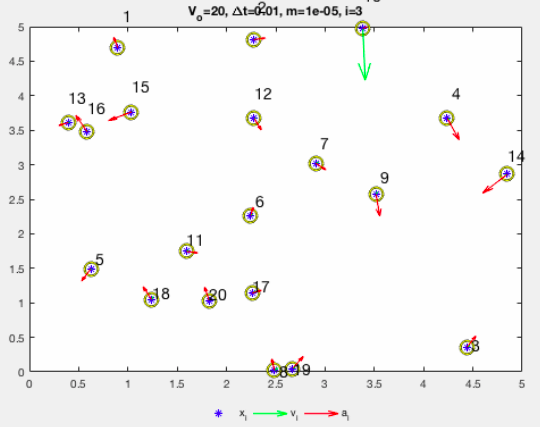
\includegraphics[width = 2in]{3.png}\\
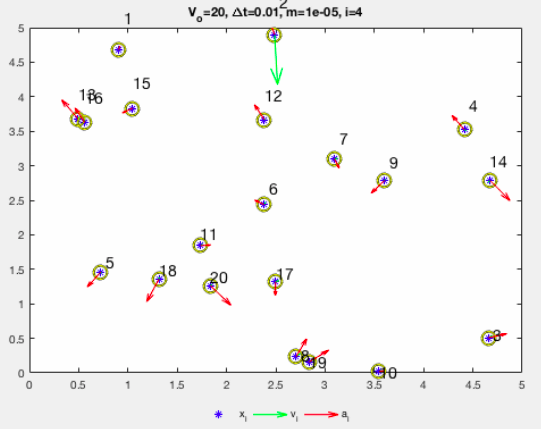
\includegraphics[width = 2in]{4.png}&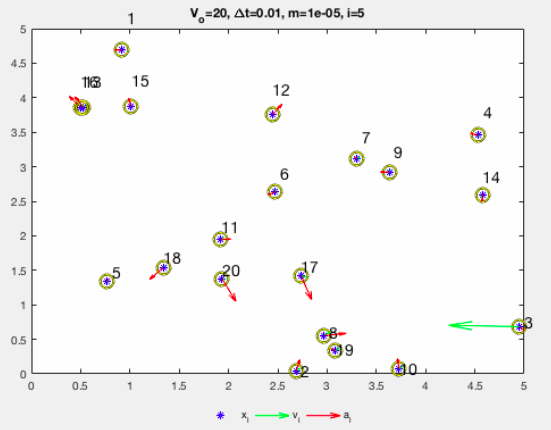
\includegraphics[width = 2in]{5.png}&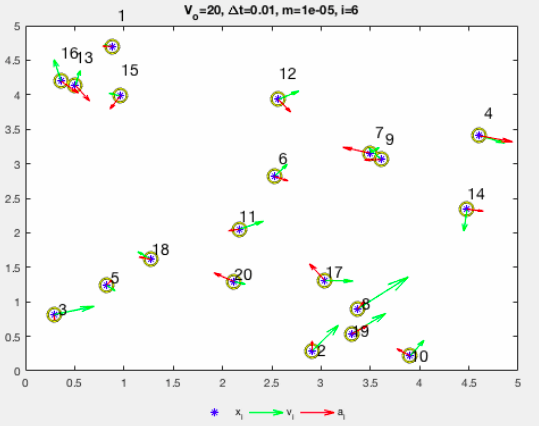
\includegraphics[width = 2in]{6.png}\\
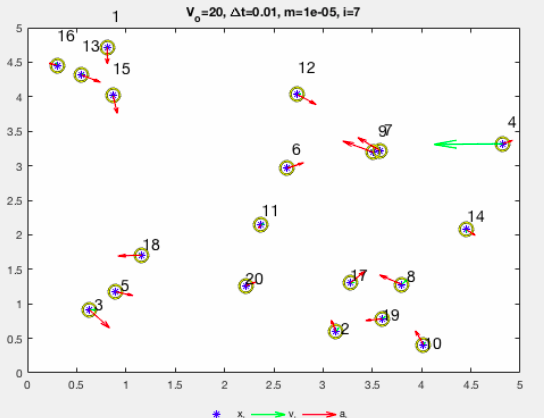
\includegraphics[width = 2in]{7.png}&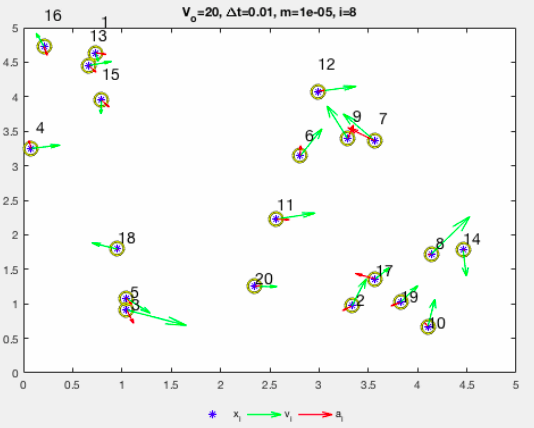
\includegraphics[width = 2in]{8.png}&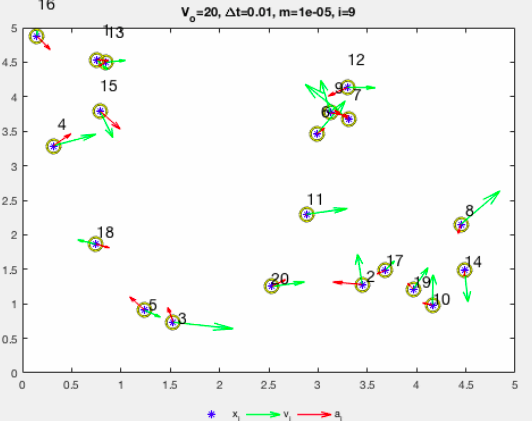
\includegraphics[width = 2in]{9.png}\\
\end{tabular}
\end{center}
The images above following the order of left to right then top to bottom. The green arrows indicate velocity and the red arrows indicate acceleration for each of the particles. Please visit the GitHub repository at \hyperlink{https://github.com/dsherma7/Computing/tree/master/MolecularDynamics/gif}{https://github.com/dsherma7/Computing/tree/master/MolecularDynamics/gif} to see .gif files illustrating the evolution of systems with various $v_0, N,$ and $\Delta t$ values to properly illustrate the dynamics of the Argon particles.

\subsection{Reducing Complexity}
In order the reduce the complexity we make one assumption and one observation. Firstly, since $f_{ij}$ is the force on particle $i$ by particle $j$, it must be true that $|f_{ji}| = |f_{ij}|$. Thus we can store the computed $f_{ij}$ for $i<j$ and replace $f_{ij}$ for $i > j$ with these stored values after accounting for the change in direction of the force.  Moreover, since the force decays with distance exceptionally fast we assume that $f_{ij} = 0$ for particles with distance greater than $3\sigma$, or 3 Van der Waal's radii. The MATLAB code at the end of this report illustrates these adjustments for $f_{ij}=f(x)$


\pagebreak
\subsection{Distribution of Particles}

In Molecular Dynamics the distribution of speeds is defined by the following function 
\begin{align*}
P(v) = C\frac{v^2}{K_BT}\exp \frac{-mv^2}{K_BT}
\end{align*}
and by the equipartition theorem we can compute $K_BT$ through the kinetic energy, and without knowing the temperature as
\begin{align*}
K_BT = \frac{m}{2}\braket{ v_x^2 + v_y^2 }
\end{align*}
where $\braket{ x} = E[x]$ is the expected value of $x$. We compared the distribution of the standardized velocity values obtained by the system shown in part (2) to the value for $P(v)$ as shown below.
\begin{center}
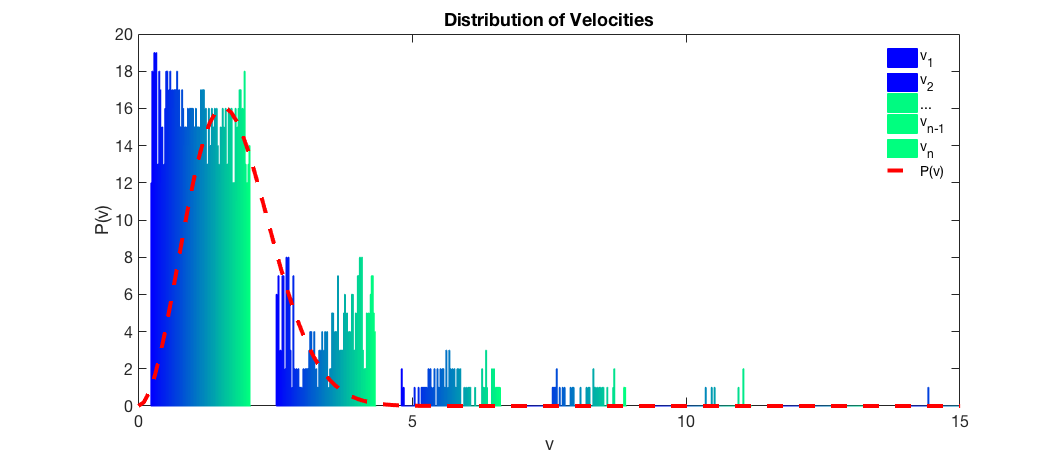
\includegraphics[width = 6in]{distibutionV.png}\\
\begin{scriptsize}
{\bf \stepcounter{graphics}\arabic{graphics}.} The comparison of the known distribution of speeds for a set of particles to the actual distribution of speeds.
\end{scriptsize}
\end{center}

We see that the velocities peak at about $1$ standard deviation, and then decay rapidly. This behavior mimics the expected distribution of speeds as defined in the equation above. 

\section{Code} 
The MATLAB code used in this assignment is given below
\lstinputlisting[language=Matlab]{../f.m}
\lstinputlisting[language=Matlab]{../a.m}
\lstinputlisting[language=Matlab]{"../plot_points.m"}
\lstinputlisting[language=Matlab]{"../print_gif.m"}


\end{document}